\documentclass{article}
\usepackage[utf8]{inputenc}
\usepackage{amsmath}
\usepackage{graphicx}
\usepackage{wrapfig}
\graphicspath{{./img/}}


\title{
Honors Project 1:\\ 
Newton's Law of Cooling and Mr. Potato Head
}
\author{Author: Rafael Betita\\Members: Quan Vu, Alex Quintanar\\ Potato \#8}

\date{April 2, 2019}

\begin{document}

\maketitle


\newpage
\section{Preamble}

During one faithful morning on the way to our Calculus class, we heard screams of panic coming directly from R216! As the students rushed on over, we found Mr. Potato Head staging a protest right in our very own classroom. In a fit of rage and protest, the suspect had strewn all "hot potatoes" around the classroom to dissuade us from eating the potatoes. Unfortuantely for him, hot potatoes are exactly what hungry students love to eat! While most students were distracted by their hunger, it seems that there was more to the mystery. A strange envelope on the teacher's desk labeled \textbf{TOP SECRET RADIOACTIVE \textit{Lancerlite}} was left empty. What could this mean?\\\newline
As Pasadena City College's brightest Calculus II students, we have been tasked by the campus police to solve two problems: when the suspicious hot potatoes were been cooked as well as the mystery of the stolen \textbf{\textit{Lancerlite}}. Using our knowledge of differential equations we will procedurally derive each solution from Newton's Law of Cooling and the Exponential Rate of Decay in order to solve these problems. With our solutions, we will be able to ascertain as to exactly when the potatoes were cooked which will lead us to exactly when our suspect, Mr. Potato Head, stole the radioactive \textbf{\textit{Lancerlite}}!

\section{The Potato Incident}

At approximately 10am, we find ourselves upon a peculiar incident. Our suspect Mr. Potato Head had dispatched a number of "hot potatoes" to prevent the hungry students of MATH005BH from eating them. Unbeknownst to him, hot potatoes are considered a delicacy amongst the students. As we bide our time waiting for the hot potatoes to cool, we decide to take some measurements to put our differential skills to the test. With enough data points, we should be able to ascertain as to when the potatoes have been cooked! 

\subsection{Newton's Law of Cooling}

As we all know, the rate of cooling for an object is directly proportional to the difference in temperature for an object and it's surroundings. This is otherwise known as Newton's Law of Cooling.


\begin{align*}
    \frac{dT}{dt}=k(T-T_s) \\
\end{align*}
\begin {center}
	\begin{tabular}{c|c}
	     Variables & Definition  \\ \hline
	     $dT$ & \text{Rate of change in Temperature} \\\hline 
	     $dt$ & \text{Rate of change in time} \\\hline
	     $k$ & \text{Cooling constant (rate of growth)} \\\hline
	     $T_s$ & \text{Temperature (of surrounding)}\\\hline
	\end{tabular}
\end{center}
\newpage
\subsection{Solving our Differential Equation}
Using Newton's Law of Cooling, our goal is to find a solution for the differential equation. This is done by undoing the differential equation using integrals. Steps are as follows.

\begin{align}
    \frac{dT}{dt}&=k(T-T_s) \\[1em]
    \frac{dT}{(T-T_s)} &= k(dt) \\[1em]
    \int \frac{dT}{(T-T_s)} &= \int k(dt)\\[1em]
    \ln|T-T_s|+C_1 &= kt+C_2\\[1em]
    \ln|T-T_s| &= kt+C\\[1em]
    e^{\ln|T-T_s|} &= e^{kt+C}\\[1em]
    |T-T_s| &= e^{c}e^{kt}\\[1em]
    |T-T_s| &= Ce^{kt}
\end{align}

We find our solution to be $\boxed{|T-T_s| = Ce^{kt}}$. Which we can use to solve for $k$, the rate of growth. As it stands, we have almost all the information we need to start solving for our missing variables ($k$) and ($C$). By using the property ($e^{k\cdot 0}, = 1 $) we can find our constant value which inevitably allows us to solve for $k$. Steps will be detailed below.


\subsection{Measurements}
Where $T_s$  (room temperature) is considered to be at $73^{\circ}$:
\begin{center}
    \begin{tabular}{|c|c|c|c|}
    \hline
    $t$ (min) & $T$ (potato) & $|T-T_s|$ & $\ln(T-T_s)$  \\\hline
    $0$ & $148.2^{\circ} F$ & $148.2 - 73.0 = 75.2$ & $4.32$ \\\hline  
    $10$ & $143.0^{\circ} F$ & $70.0$ & $4.25$ \\\hline
    $20$ & $138.7^{\circ} F$ & $65.7$ & $4.19$ \\\hline
    $30$ & $133.9^{\circ} F$ & $60.9$ & $4.11$ \\\hline
    $40$ & $128.8^{\circ} F$ & $55.8$ & $4.02$ \\\hline
    $50$ & $125.8^{\circ} F$ & $52.8$ & $3.97$ \\\hline
    $60$ & $122.5^{\circ} F$ & $49.5$ & $3.90$\\\hline
    \end{tabular}\\[1em]
\end{center}
\begin{center}
    Where $t$ = time, $T$ = temperature, $T_s$ = surrounding temperature
\end{center}
\newpage

\subsection{Solving for our missing variables}
As mentioned previously, now that we have the solution to our differential equation, we can start plugging in values. at $t = 0$, we are able to easily find our constant as such:

\begin{align}
    |T-T_s| &= Ce^{kt}\\[1em]
    |148.2-73.0| &= Ce^{k\cdot 0}\\[1em]
    C(1) &= 75.2
\end{align}

We find our constant to be 75.2. Now we can start solving for our rate of growth, $k$.\\

Given that $t = 10$ and $C = 75.2$:
\begin{align}
    |143.0-73.0| &= 75.2e^{k\cdot 10}\\[1em]
    \frac{70}{75.2} &= e^{k\cdot 10}\\[1em]
    \ln{(.93)} &= \ln{(e^{k\cdot 10})}\\[1em]
    -0.0717 &= k \cdot 10 \\[1em]
    -0.00717 &= k
\end{align}
We find our rate of growth to be approximately \boxed{k\approx-0.0071} . We will further verify our findings in the next section below using linear regression modelling.

\subsection{Graph}
Using linear regression modelling, we interpolate our data onto Desmos. Upon closer insepection, we find our slope to be around $-0.00710714$ on Desmos, very close to our own calculation of $k$. This value can also be expressed by rearranging our original equation as follows:
\begin{align}
    \ln|T-T_s| &= kt+C\\
    \frac{\ln|T-T_s|}{t}+C &=k
\end{align}

\newpage
Furthermore, we verify our derived solution for Newton's Law of Cooling by plotting $T$ (temperature) over $t$ against our own linear equation of $\boxed{|T-T_s| = Ce^{kt}}$.\\



\begin{figure}[t]
\centering
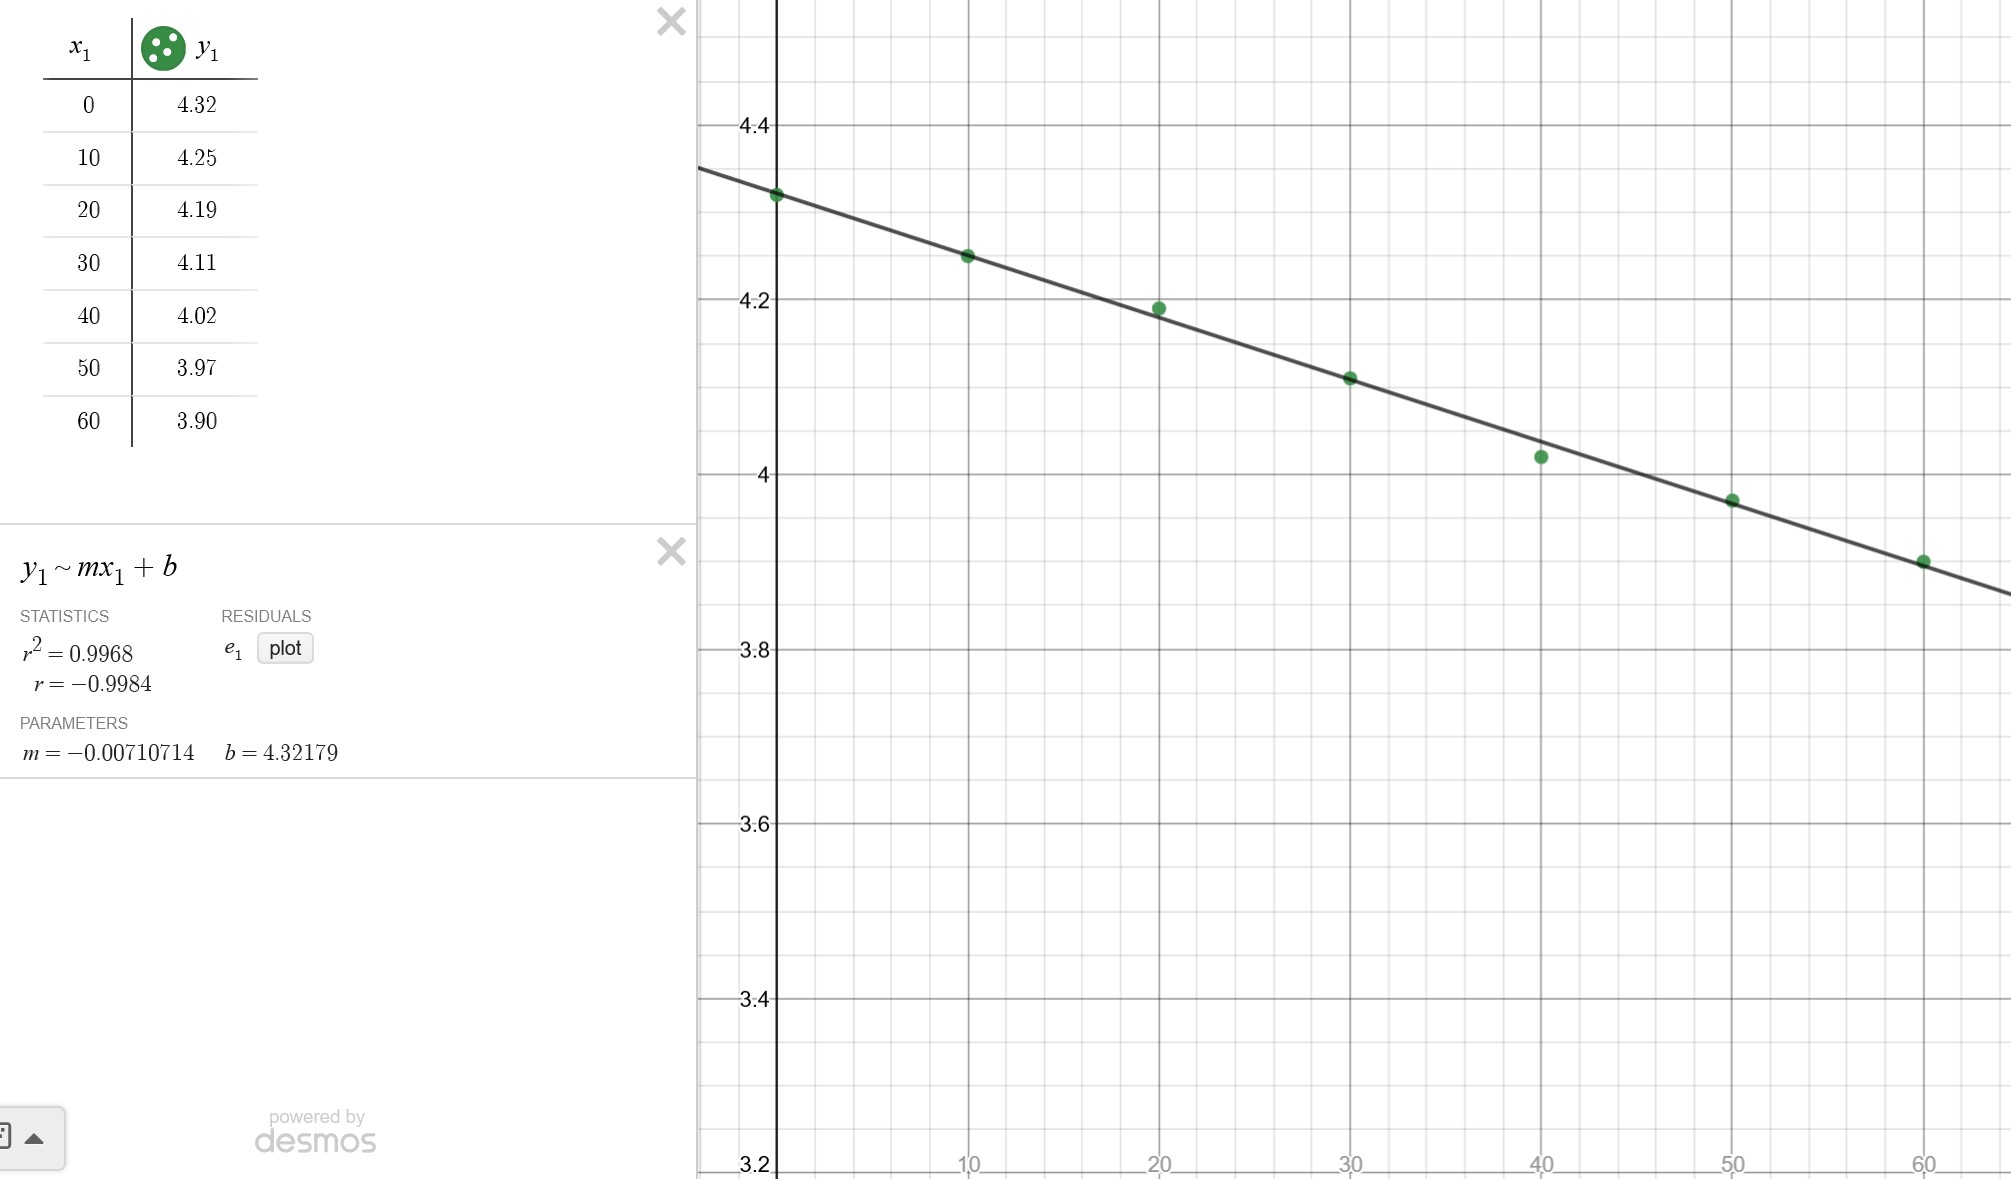
\includegraphics[width=0.8\textwidth]{graph.jpg}
\caption{Our data points plotted using Desmos.}
    \label{fig:my_label}
\end{figure}

\begin{figure}[h]
    \centering
    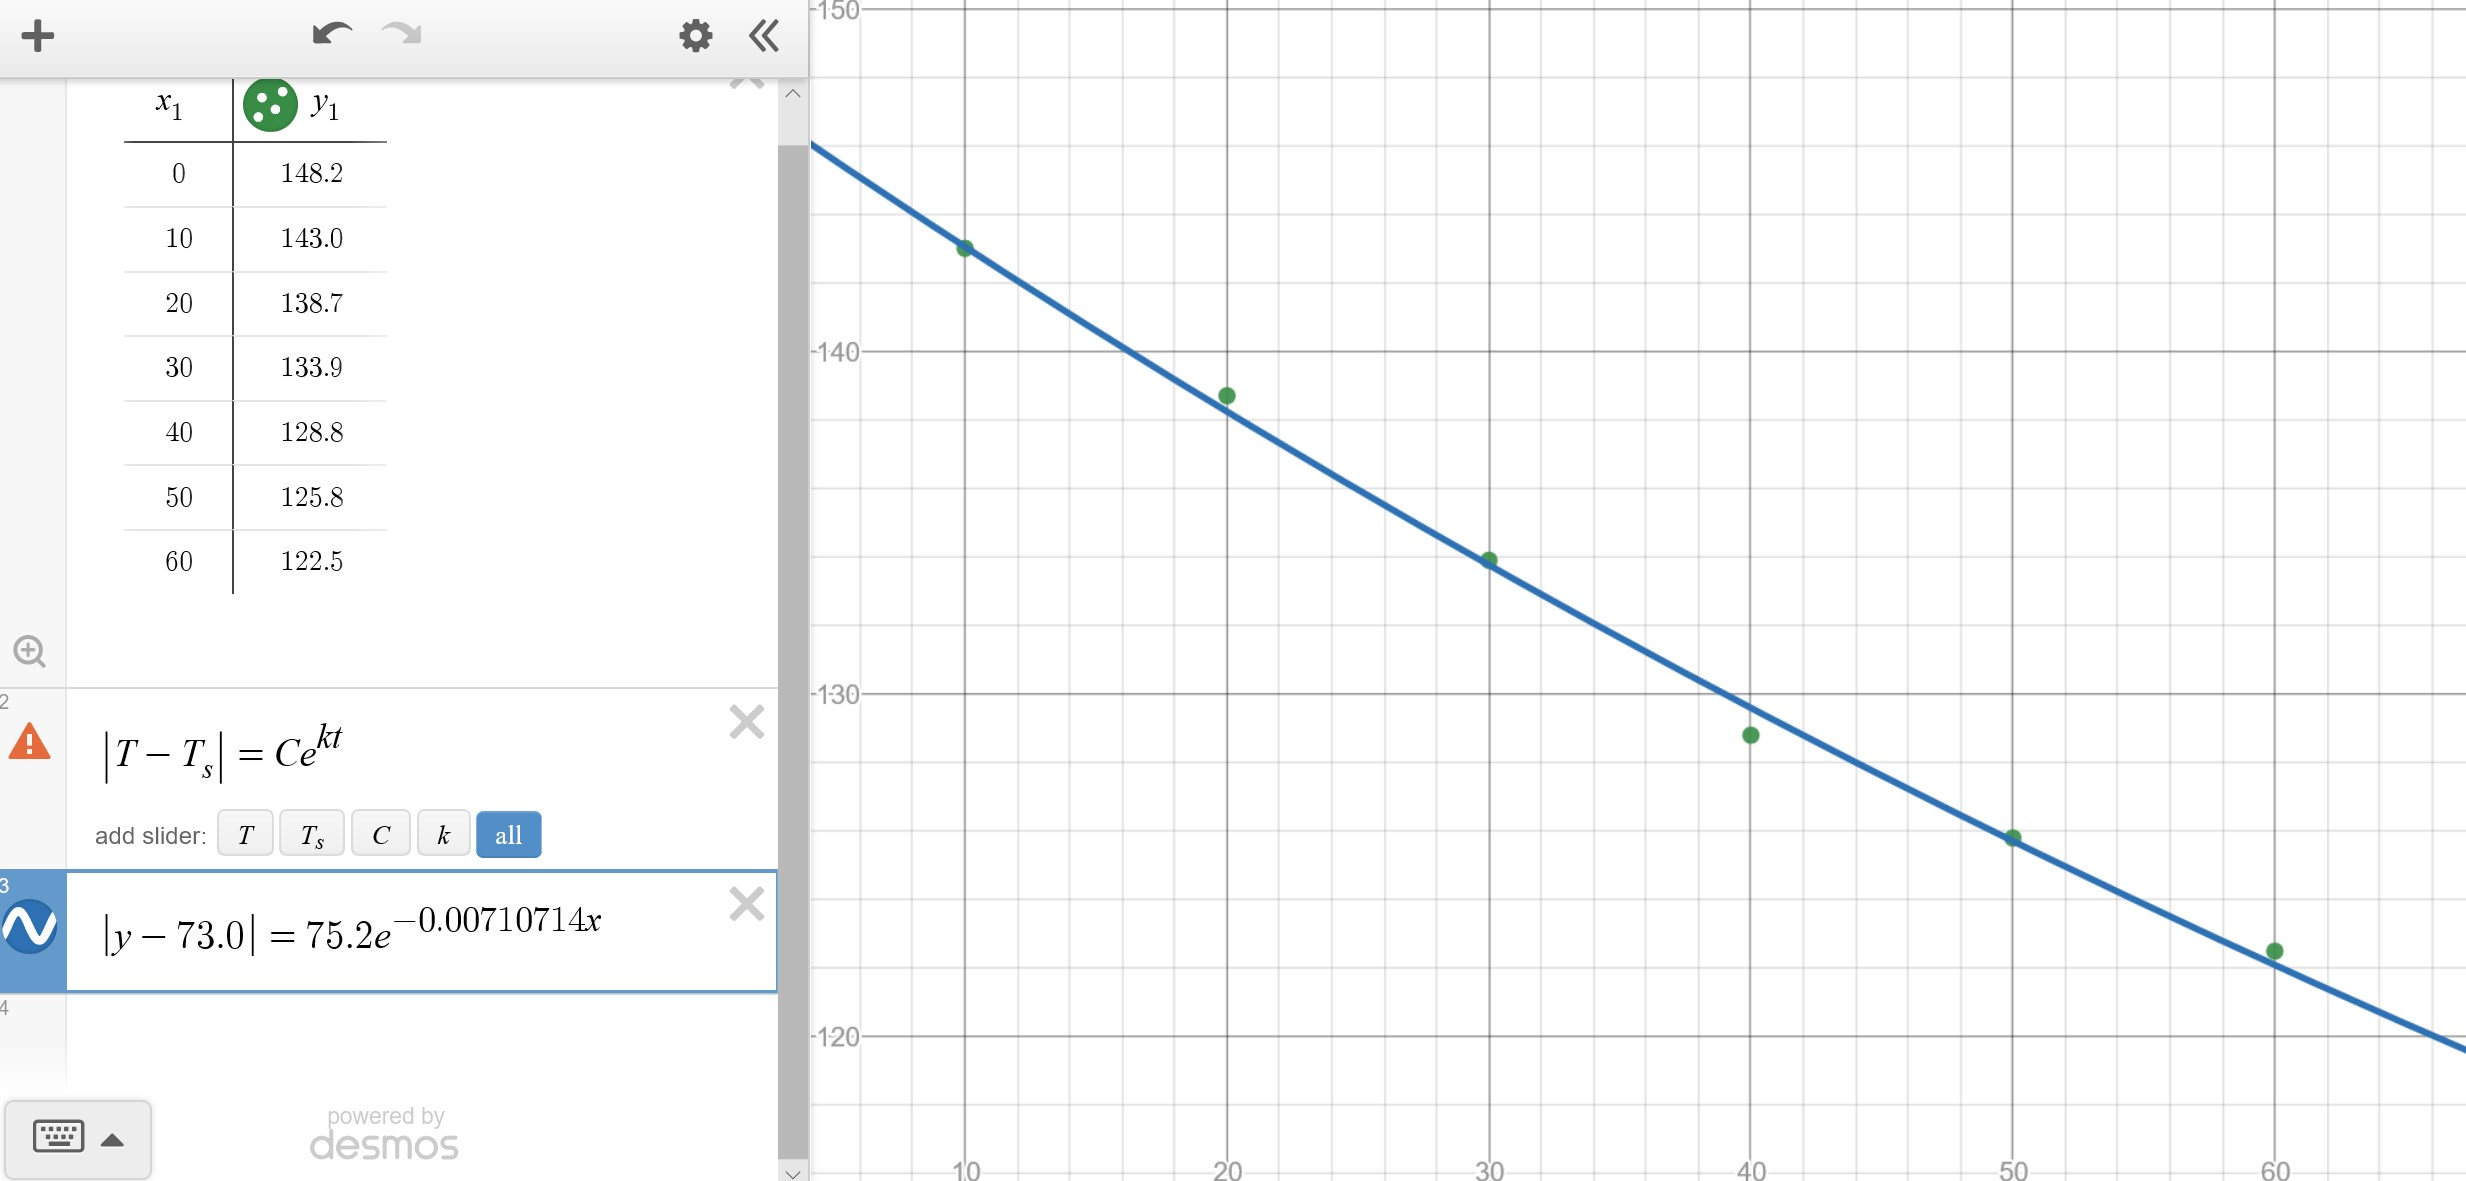
\includegraphics[width=0.8\textwidth]{Tvst.jpg}
    \caption{Graph of Temperature over time against our derived equation}
    \label{fig:my_label}
\end{figure}

The graphs reflects a direct correlation between the collected data points and the derived equation (as shown in blue).

\newpage
\subsection{Calculations}
With all of our missing variables ($C$, $k$) found, we can proceed to find out just exactly when our potato was cooked ($t$). Now, given that a fully cooked potato starts at $208^\circ\text{F}$, we solve for $t$ using our equation as follows:
\begin{align}
    |T-T_s| &= Ce^{kt}\\[1em]
    |208 - 73| &= 75.2e^{-0.0071\cdot t}\\[1em]
    |135| &=  75.2e^{-0.0071\cdot t}\\[1em]
    \frac{135}{75.2} &= e^{-0.0071\cdot t}\\[1em]
    \ln{\left(\frac{135}{75.2}\right)} &= \ln{\left(e^{-0.0071\cdot t}\right)}\\[1em]
    -0.59 &= -0.0071\cdot t\\[1em]
    t &= -82.41
\end{align}
We find that the time elapsed since the potato was $208^\circ$F was approximately 82 minutes ago. This is roughly around 1 hour and 13 minutes upon first measuring the temperature of the potato at 10am, making the time of cooking at around \boxed {8:47\text{am}} . Seems like our potato friend is quite an early riser! We can confirm by evaluating other test points.\\ 

Given $t=30$:
\begin{align}
    T_{30}-73 &= 75.2e^{-.0071\cdot(30)}\\
    T_{30}-73 &= 75.2(.808)\\
    T_{30} &= 73+60.77\\
    T_{30} &= 133.77
\end{align}


\text{Given $t=60$:}
\begin{align}
    T_{60}-73 &= 75.2e^{-.0071\cdot(60)}\\
    T_{60}-73 &= 75.2(.653)\\
    T_{60} &= 73+49.11\\
    T_{60} &= 122.11
\end{align}

Both answers support our collected measurements!

\newpage
\subsection{Analysis}
Now, while our calculations seem to agree, for the temperature of this particular potato to last so long we have to take a few things into consideration.\\

\begin{wrapfigure}[24]{r}{0.32\textwidth}
    \centering
    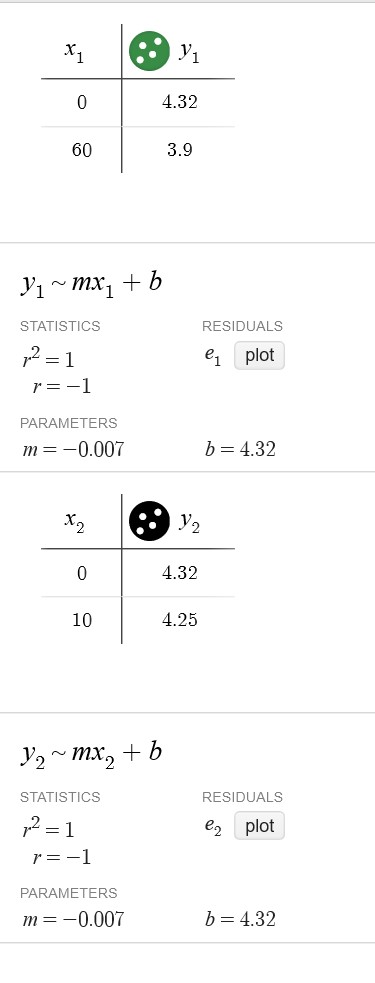
\includegraphics[height=.5\textheight]{extra.jpg}
    \caption{Testing regression with less data points.}
\end{wrapfigure}

We postulate: Will the number of collected points affect the overall estimated growth rate? As evident from the figure to the right, leaving all but two points still results in an approximate growth rate of $-0.0071$. Thus our findings lead us to believe that it is entirely possible for the potatoes to have been cooked an hour or so prior to their discovery. \\

Some other considerations: One way that the data could have been skewed is based on the
temperature of the surroundings. Since we found our potatoes to be well secured its foil
container, we are left to think about the role of the surrounding temperature within our
calculations. We are entirely under the assumption that our potato has been sitting in a room
of $73^{\circ}F$. It is entirely possible that the potato could have possibly been transported
 from different surroundings with different temperatures. Either
way, at this point it is mere conjecture and is left up to the reader's own imagination. We now
move on to our second problem at hand.

\newpage
\section{The Mystery of the Missing Lancerlite}
As the faithful students of MATH005BH, it is our responsibility to solve once and for all the mystery of the missing \textbf{\textit{Lancerlite}}. While there isn't much we can do about the missing \textbf{\textit{Lancerlite}}, we can however determine how many hours until the \textbf{\textit{Lancerlite}} becomes explosive. 

\subsection{Exponential Decay}
We will yet again derive our solution, but this time using our knowledge of exponential decay. Given that the rate of growth/decay is proportional the the remaining mass, we express this relationship as follows:


\begin{align*}
    \frac{dM}{dt}=k(M_0) \qquad\qquad
    \begin{tabular}{c|c}
     Variables & Definition  \\ \hline
     $dM$ & \text{Rate of change in mass} \\\hline 
     $dt$ & \text{Rate of change in time} \\\hline
     $k$ & \text{Rate of decay} \\\hline
     $M_0$ & \text{Initial Mass}\\\hline
\end{tabular}
\end{align*}

\subsection{Solving our Differential Equation}
Just like in Newton's Law of Cooling, our goal is to find a solution for the given differential equation. This is done by undoing the differential equation using integrals. Steps are as follows.

\begin{align}
    \frac{dM}{dt}&=k(M_0) \\[1em]
    \frac{dM}{M_0} &= k(dt) \\[1em]
    \int \frac{dM}{M_0} &= \int k(dt)\\[1em]
    \ln|M_0|+C_1 &= kt+C_2\\[1em]
    \ln|M_0| &= kt+C\\[1em]
    e^{\ln|M_0|} &= e^{kt+C}\\[1em]
    |M_0| &= e^{c}e^{kt}\\[1em]
    |M_0| &= Ce^{kt}
\end{align}

We find our solution to be $\boxed{|M_0| = Ce^{kt}}$.

\subsection{Calculations}
Now that we have a solution to our differential equation,  we can now use it to solve for $k$, the rate of growth. Very much like the first problem, we start by solving for our constant at $t = 0$.\\\\
Given the assumption that mass of the \textbf{\textit{Lancerlite}} is at 1 (100\%) at $t = 0$:
\begin{align}
    1 &= Ce^{k(0)}\\
    1 & = C(1)
\end{align}

Since we find that \boxed{$C = 1$} our constant be cancelled out from the original equation:
\begin{align}
    M = e^{kt}    
\end{align}
To determine the rate of growth, we need to be able to compare another test point from our initial mass. Luckily, our suspect was kind enough to give us a clue: ``The half-life of \textbf{\textit{Lancerlite}} (in hours) is equal to one fifth the number formed by the last two digits of the first year that Jackie Robinson attended PCC.'' Being the resourceful students that we are, we find that that exact year to be 1937. Using that information we get the half-life in hours to be $\frac{37}{5} = 7.4$ hours! We can now solve for our rate of growth, using $M_{7.4} = .50$.\\

Given that the half-life represents 50\% of the mass, we take M to be 0.5:
\begin{align}
    M &= e^{kt}\\[1em]
    .50 &= e^{k7.4}\\[1em]
    \ln(.50) &= \ln(e^{7.4k})\\[1em]
    -0.69 &= 7.4k \\[1em]
    k &= -0.093
\end{align}
Now that k is solved for, we can now fully solve for our missing variable $t$. We were informed by the authorities that the \textbf{\textit{Lancerlite}} becomes explosive at 35\% of its original amount. To calculate the time it takes to decay up to that point, we reuse our equation where $M = .35$ with $k = -0.093$ :
\begin{align}
    M &= e^{kt}\\[1em]
    .35 &= e^{-0.093t}\\[1em]
    \ln(.35) &= \ln(e^{-0.093t})\\[1em]
    -1.04 &= -0.093t \\[1em]
    t &= 11.28
\end{align}
Since we used $t$ as hours to determine our k, we get $t$ as the time in hours. We make a quick conversion for .28 hours to minutes as follows:
\begin{align}
	\frac{.28 \text{ hour}}{1} \times \frac{60 \text{ minutes}}{\text{hour}} \approx 16.8 \text{ minutes}
\end{align}
At approximately 11 hours and 17 minutes from the time the \textbf{\textit{Lancerlite}} was stolen, it would have decayed to about 35\% of its mass and become explosive! Given that the \textbf{\textit{Lancerlite}} was removed from its laboratory storage 30 minutes after the potatoes were cooked (8:47am), that would only give the authorities until around 8:30pm to nab that potato fiend! Oh, wait a minute..

\end{document}
